\section{FPGA Architecture History}
Before any work can begin on an FPGA placer, it is necessary to understand both the objects being placed and the medium in which they are placed.
Configurable logic devices have undergone significant evolution over the past four decades. 
We will briefly review the evolution of configurable logic architecture starting in the 1970s and quickly work our way up to modern day FPGA architecture. 

\textbf{PLA:} \quad
The journey began with the Programmable Logic Array (PLA) in the early 1970s. 
The PLA implemented output logic using a programmable-OR and programmable-AND plane that formed a sum-of-products equation for each output through programmable fuses. 
Around the same time, the Programmable Array Logic (PAL) was introduced. 
The PAL simplified the PLA by fixing the OR gates, resulting in a fixed-OR, programmable-AND design, which sacrificed some logic flexibility to simplify its manufacture. 
Figure \ref{fig:pal_2} shows one such PAL architecture. 

\textbf{CPLD:} \quad 
Later in the same decade came the Complex Programmable Logic Device (CPLD), which took the form of an array of Configurable Logic Blocks (CLBs). 
These CLBs were typically modified PAL blocks that included the PAL itself along with macrocells such as flip-flops, multiplexers, and tri-state buffers. 
The CPLD functioned as an array of PALs connected by a central programmable switch matrix and could be programmed using a hardware description language (HDL) like VHDL. 
Figure \ref{fig:cpld} shows one such CPLD architecture. 
\\

{
    \centering
    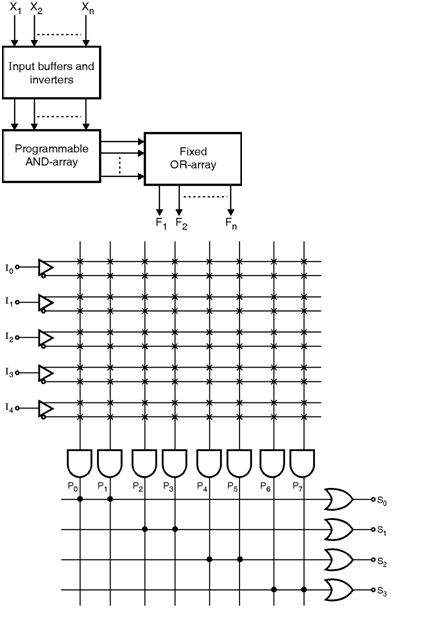
\includegraphics[width=\columnwidth]{figures/pal_2.png}
    \captionof{figure}{PAL architecture with 5 inputs, 8 programmable AND gates and 4 fixed OR gates}
    \label{fig:pal_2}
    % https://www.electronics-tutorial.net/Programmable-Logic-Device-Architectures/Programmable-Logic-Devices/Programmable-Array-Logic-PAL/
    % https://www.naukri.com/code360/library/difference-between-pla-and-pal 
}

\newcolumn

\textbf{Homogeneous FPGA:} \quad 
The mid-1980s saw the introduction of homogeneous FPGAs, which were built as a grid of CLBs. 
Rather than using a central programmable switch matrix as in CPLDs, FPGAs adopted an island style architecture in which each CLB is surrounded on all sides by programmable routing resources, as shown in Figure \ref{fig:homogen_fpga}. 
The first commercially viable FPGA, produced by Xilinx in 1984, featured 16 CLBs arranged in a 4x4 grid. 
As FPGA technology advanced, CLBs were redesigned to use lookup tables (LUTs) instead of PAL arrays for greater logic density. 
The capacity of an FPGA was often measured by how many logical elements or CLBs it offered, which grew from hundreds to thousands and now to hundreds of thousands of CLBs.
\\ 

{
    \centering
    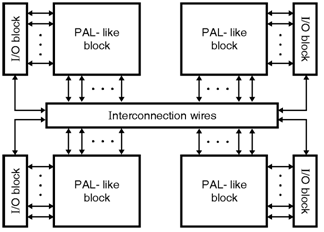
\includegraphics[width=0.8\columnwidth]{figures/cpld.png}
    \captionof{figure}{CPLD architecture with 4 CLBs (PAL-like blocks)}
    \label{fig:cpld}
    % https://www.electronics-tutorial.net/Programmable-Logic-Device-Architectures/CPLD/Complex-Programmable-Logic-Device-CPLDs/
}
{
    \centering
    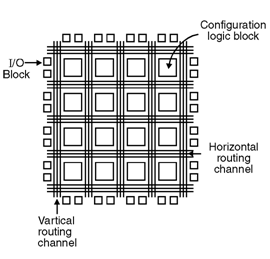
\includegraphics[width=\columnwidth]{figures/homogenous_fpga.png}
    \captionof{figure}{A homogeneous island-style FPGA architecture with 16 CLBs in a grid.}
    \label{fig:homogen_fpga}
    % https://www.electronics-tutorial.net/Programmable-Logic-Device-Architectures/FPGA/Field-programmable-gate-array-FPGA/
}

\newpage

{
    \centering
    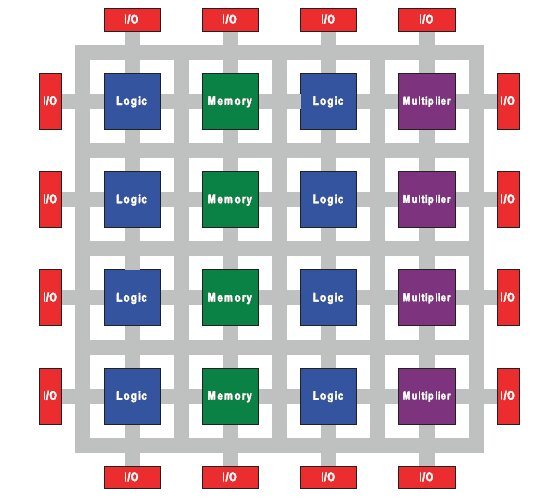
\includegraphics[width=\columnwidth]{figures/heterogenous_fpga_3.jpg}
    \captionof{figure}{A heterogeneous island-style FPGA with a mix of CLBs and macrocells.}
    \label{fig:heterogen_fpga}
    % https://www.electronics-tutorial.net/Programmable-Logic-Device-Architectures/FPGA/Field-programmable-gate-array-FPGA/
}
\vspace{0.25cm}

\textbf{Heterogenous FPGA:} \quad 
This brings us to modern day FPGA architectures. 
To meet the needs of increasingly complex designs, FPGA vendors introduced heterogeneous FPGAs. 
In these devices, hard macros such as Block RAM (BRAM) and Digital Signal Processing (DSP) slices are integrated into the programmable logic fabric along with CLBs, like shown in Figure \ref{fig:heterogen_fpga}. 
This design enables the direct instantiation of common subsystems like memories and multipliers, without having to recreate them from scratch using CLBs. 
Major vendors such as Xilinx (AMD) and Altera (Intel) now employ heterogeneous island-style architectures in their devices. 
As designs become increasingly large and complex, FPGAs meet the demand by becoming increasingly heterogenous, incorporating a wider variety of hard macros into the fabric. 

